\documentclass[ignorenonframetext,]{beamer}
\setbeamertemplate{caption}[numbered]
\setbeamertemplate{caption label separator}{: }
\setbeamercolor{caption name}{fg=normal text.fg}
\beamertemplatenavigationsymbolsempty
\usepackage{lmodern}
\usepackage{amssymb,amsmath}
\usepackage{ifxetex,ifluatex}
\usepackage{fixltx2e} % provides \textsubscript
\ifnum 0\ifxetex 1\fi\ifluatex 1\fi=0 % if pdftex
  \usepackage[T1]{fontenc}
  \usepackage[utf8]{inputenc}
\else % if luatex or xelatex
  \ifxetex
    \usepackage{mathspec}
  \else
    \usepackage{fontspec}
  \fi
  \defaultfontfeatures{Ligatures=TeX,Scale=MatchLowercase}
\fi
\usetheme[]{AnnArbor}
\usecolortheme{beaver}
\usefonttheme{structurebold}
% use upquote if available, for straight quotes in verbatim environments
\IfFileExists{upquote.sty}{\usepackage{upquote}}{}
% use microtype if available
\IfFileExists{microtype.sty}{%
\usepackage{microtype}
\UseMicrotypeSet[protrusion]{basicmath} % disable protrusion for tt fonts
}{}
\newif\ifbibliography
\hypersetup{
            pdftitle={Séance 5.2: Paramètres de variation},
            pdfauthor={Visseho Adjiwanou, PhD.},
            pdfborder={0 0 0},
            breaklinks=true}
\urlstyle{same}  % don't use monospace font for urls
\usepackage{color}
\usepackage{fancyvrb}
\newcommand{\VerbBar}{|}
\newcommand{\VERB}{\Verb[commandchars=\\\{\}]}
\DefineVerbatimEnvironment{Highlighting}{Verbatim}{commandchars=\\\{\}}
% Add ',fontsize=\small' for more characters per line
\usepackage{framed}
\definecolor{shadecolor}{RGB}{248,248,248}
\newenvironment{Shaded}{\begin{snugshade}}{\end{snugshade}}
\newcommand{\KeywordTok}[1]{\textcolor[rgb]{0.13,0.29,0.53}{\textbf{#1}}}
\newcommand{\DataTypeTok}[1]{\textcolor[rgb]{0.13,0.29,0.53}{#1}}
\newcommand{\DecValTok}[1]{\textcolor[rgb]{0.00,0.00,0.81}{#1}}
\newcommand{\BaseNTok}[1]{\textcolor[rgb]{0.00,0.00,0.81}{#1}}
\newcommand{\FloatTok}[1]{\textcolor[rgb]{0.00,0.00,0.81}{#1}}
\newcommand{\ConstantTok}[1]{\textcolor[rgb]{0.00,0.00,0.00}{#1}}
\newcommand{\CharTok}[1]{\textcolor[rgb]{0.31,0.60,0.02}{#1}}
\newcommand{\SpecialCharTok}[1]{\textcolor[rgb]{0.00,0.00,0.00}{#1}}
\newcommand{\StringTok}[1]{\textcolor[rgb]{0.31,0.60,0.02}{#1}}
\newcommand{\VerbatimStringTok}[1]{\textcolor[rgb]{0.31,0.60,0.02}{#1}}
\newcommand{\SpecialStringTok}[1]{\textcolor[rgb]{0.31,0.60,0.02}{#1}}
\newcommand{\ImportTok}[1]{#1}
\newcommand{\CommentTok}[1]{\textcolor[rgb]{0.56,0.35,0.01}{\textit{#1}}}
\newcommand{\DocumentationTok}[1]{\textcolor[rgb]{0.56,0.35,0.01}{\textbf{\textit{#1}}}}
\newcommand{\AnnotationTok}[1]{\textcolor[rgb]{0.56,0.35,0.01}{\textbf{\textit{#1}}}}
\newcommand{\CommentVarTok}[1]{\textcolor[rgb]{0.56,0.35,0.01}{\textbf{\textit{#1}}}}
\newcommand{\OtherTok}[1]{\textcolor[rgb]{0.56,0.35,0.01}{#1}}
\newcommand{\FunctionTok}[1]{\textcolor[rgb]{0.00,0.00,0.00}{#1}}
\newcommand{\VariableTok}[1]{\textcolor[rgb]{0.00,0.00,0.00}{#1}}
\newcommand{\ControlFlowTok}[1]{\textcolor[rgb]{0.13,0.29,0.53}{\textbf{#1}}}
\newcommand{\OperatorTok}[1]{\textcolor[rgb]{0.81,0.36,0.00}{\textbf{#1}}}
\newcommand{\BuiltInTok}[1]{#1}
\newcommand{\ExtensionTok}[1]{#1}
\newcommand{\PreprocessorTok}[1]{\textcolor[rgb]{0.56,0.35,0.01}{\textit{#1}}}
\newcommand{\AttributeTok}[1]{\textcolor[rgb]{0.77,0.63,0.00}{#1}}
\newcommand{\RegionMarkerTok}[1]{#1}
\newcommand{\InformationTok}[1]{\textcolor[rgb]{0.56,0.35,0.01}{\textbf{\textit{#1}}}}
\newcommand{\WarningTok}[1]{\textcolor[rgb]{0.56,0.35,0.01}{\textbf{\textit{#1}}}}
\newcommand{\AlertTok}[1]{\textcolor[rgb]{0.94,0.16,0.16}{#1}}
\newcommand{\ErrorTok}[1]{\textcolor[rgb]{0.64,0.00,0.00}{\textbf{#1}}}
\newcommand{\NormalTok}[1]{#1}
\usepackage{longtable,booktabs}
\usepackage{caption}
% These lines are needed to make table captions work with longtable:
\makeatletter
\def\fnum@table{\tablename~\thetable}
\makeatother
\usepackage{graphicx,grffile}
\makeatletter
\def\maxwidth{\ifdim\Gin@nat@width>\linewidth\linewidth\else\Gin@nat@width\fi}
\def\maxheight{\ifdim\Gin@nat@height>\textheight0.8\textheight\else\Gin@nat@height\fi}
\makeatother
% Scale images if necessary, so that they will not overflow the page
% margins by default, and it is still possible to overwrite the defaults
% using explicit options in \includegraphics[width, height, ...]{}
\setkeys{Gin}{width=\maxwidth,height=\maxheight,keepaspectratio}

% Prevent slide breaks in the middle of a paragraph:
\widowpenalties 1 10000
\raggedbottom

\AtBeginPart{
  \let\insertpartnumber\relax
  \let\partname\relax
  \frame{\partpage}
}
\AtBeginSection{
  \ifbibliography
  \else
    \let\insertsectionnumber\relax
    \let\sectionname\relax
    \frame{\sectionpage}
  \fi
}
\AtBeginSubsection{
  \let\insertsubsectionnumber\relax
  \let\subsectionname\relax
  \frame{\subsectionpage}
}

\setlength{\parindent}{0pt}
\setlength{\parskip}{6pt plus 2pt minus 1pt}
\setlength{\emergencystretch}{3em}  % prevent overfull lines
\providecommand{\tightlist}{%
  \setlength{\itemsep}{0pt}\setlength{\parskip}{0pt}}
\setcounter{secnumdepth}{0}

\title{Séance 5.2: Paramètres de variation}
\subtitle{Extensions}
\author{Visseho Adjiwanou, PhD.}
\date{16 February 2022}

\begin{document}
\frame{\titlepage}

\begin{frame}{Plan de présentation}

\begin{itemize}
\tightlist
\item
  Scores standardisés ou scores-Z
\item
  Loi normale
\item
  Distribution d'échantillonnage
\item
  Théorème central limite
\item
  Intervalles de confiances
\item
  Application
\end{itemize}

\end{frame}

\begin{frame}{Scores standardisés ou scores-Z}

\begin{itemize}
\tightlist
\item
  Un score standardisé mesure à combien d'écarts-types de la moyenne se
  situe un score donné
\item
  Sa formule est :
\end{itemize}

\[ Z_i = \frac{X_i - \bar{X}}{s}\]

\begin{itemize}
\item
  \(Z_i\) = le score standadisé du \(i^e\) cas
\item
  \(X_i\) = le score du \(i^e\) cas
\item
  \(\bar{X}\) = la moyenne
\item
  s = l'écart-type
\item
  Ils sont particulièrement utiles lorsque l'on compare des scores
  provenant de distribution dont les moyennes et les écarts-types sont
  différentes.
\end{itemize}

\end{frame}

\begin{frame}{Scores standardisés ou scores-Z}

\begin{itemize}
\item
  Exemple: Qui de Bill avec un revenu de 80000 au Québec et Alice avec
  un revenu de 110000 à Alberta a le meilleu revenu dans sa province?
\item
  Rappelons que
\item
  le revenu moyen à Alberta 103446.28 est et l'ecart-type vaut 92722.25
\item
  le revenu moyen au Québec 71150.87 est et l'écart-type vaut 46601.69
\end{itemize}

\end{frame}

\begin{frame}[fragile]{Scores standardisés ou scores-Z}

\begin{itemize}
\tightlist
\item
  Calculons les scores standardisés de Bill et de Alice
\end{itemize}

\begin{Shaded}
\begin{Highlighting}[]
\CommentTok{# Québec}
\NormalTok{Score_z_bill <-}\StringTok{ }\NormalTok{(}\DecValTok{80000} \OperatorTok{-}\StringTok{ }\FloatTok{71150.87}\NormalTok{)}\OperatorTok{/}\FloatTok{46601.69}
\NormalTok{Score_z_bill}
\end{Highlighting}
\end{Shaded}

\begin{verbatim}
## [1] 0.1898886
\end{verbatim}

\begin{Shaded}
\begin{Highlighting}[]
\CommentTok{# Alberta}
\NormalTok{Score_z_alice <-}\StringTok{ }\NormalTok{(}\DecValTok{110000} \OperatorTok{-}\StringTok{ }\FloatTok{103446.28}\NormalTok{)}\OperatorTok{/}\FloatTok{92722.25}
\NormalTok{Score_z_alice}
\end{Highlighting}
\end{Shaded}

\begin{verbatim}
## [1] 0.0706812
\end{verbatim}

\begin{itemize}
\tightlist
\item
  On voit que Bill a un revenu qui se situe à 0.19 écart type de la
  moyenne des revenus au Québec alors qu'Alice ne se trouve qu'à 0.07
  écart-type. Donc, le revenu de Bill est meilleur que le revenu
  d'Alice.
\end{itemize}

\end{frame}

\begin{frame}{Exercice}

Voici les scores de 6 individus:

\begin{longtable}[]{@{}ll@{}}
\toprule
Individu & Score (Xi)\tabularnewline
\midrule
\endhead
1 & 64\tabularnewline
2 & 68\tabularnewline
3 & 70\tabularnewline
4 & 71\tabularnewline
5 & 69\tabularnewline
6 & 66\tabularnewline
\bottomrule
\end{longtable}

\begin{enumerate}
\def\labelenumi{\arabic{enumi}.}
\tightlist
\item
  Calculer les scores sstandardisés (Zi) de chaque individu
\item
  Calculer la moyenne des scores (Zi). Quelle conclusions tirez-vous?
\item
  Calculer l'écart-type des scores (Zi). Quelle conclusion tirez-vous?
\item
  Pouvez-vous démontrer les résultats obtenus au 2 et 3 à partir de la
  formule du score standardisé?
\end{enumerate}

\end{frame}

\begin{frame}[fragile]{Solution}

\begin{Shaded}
\begin{Highlighting}[]
\NormalTok{Score <-}\StringTok{ }\KeywordTok{c}\NormalTok{(}\DecValTok{64}\NormalTok{, }\DecValTok{68}\NormalTok{, }\DecValTok{70}\NormalTok{, }\DecValTok{71}\NormalTok{, }\DecValTok{69}\NormalTok{, }\DecValTok{66}\NormalTok{)}
\NormalTok{Score}
\end{Highlighting}
\end{Shaded}

\begin{verbatim}
## [1] 64 68 70 71 69 66
\end{verbatim}

\begin{Shaded}
\begin{Highlighting}[]
\NormalTok{Z_score <-}\StringTok{ }\NormalTok{(Score }\OperatorTok{-}\StringTok{ }\KeywordTok{mean}\NormalTok{(Score))}\OperatorTok{/}\KeywordTok{sd}\NormalTok{(Score)}
\NormalTok{Z_score}
\end{Highlighting}
\end{Shaded}

\begin{verbatim}
## [1] -1.5339300  0.0000000  0.7669650  1.1504475  0.3834825 -0.7669650
\end{verbatim}

\begin{Shaded}
\begin{Highlighting}[]
\CommentTok{# Moyenne}
\KeywordTok{mean}\NormalTok{(Z_score)}
\end{Highlighting}
\end{Shaded}

\begin{verbatim}
## [1] 0
\end{verbatim}

\begin{Shaded}
\begin{Highlighting}[]
\CommentTok{# Écart-type}
\KeywordTok{sd}\NormalTok{(Z_score)}
\end{Highlighting}
\end{Shaded}

\begin{verbatim}
## [1] 1
\end{verbatim}

\end{frame}

\begin{frame}{La distribution normale}

\begin{itemize}
\tightlist
\item
  La distribution normale est une distribution particulière, symétrique
  en forme de cloche
\item
  Ce n'est pas toutes les distributions en forme de cloche qui sont
  normales
\item
  Une distribution normale doit s'écrire sous la forme:
\end{itemize}

\[ Y = \frac{e^{-(x - \mu)^2/2\sigma^2}}{\sigma\sqrt{2\pi}}\] - \(\mu\)
est la moyenne et \(\sigma\) l'écart-type

\begin{itemize}
\tightlist
\item
  Elle est notée \(N(\mu, \sigma)\)
\end{itemize}

\end{frame}

\begin{frame}[fragile]{La distribution normale}

Voici deux distributions normales

\begin{Shaded}
\begin{Highlighting}[]
\KeywordTok{library}\NormalTok{(tidyverse)}
\end{Highlighting}
\end{Shaded}

\begin{verbatim}
## Warning: package 'tidyverse' was built under R version 3.6.2
\end{verbatim}

\begin{verbatim}
## -- Attaching packages --------------------------------------- tidyverse 1.3.1 --
\end{verbatim}

\begin{verbatim}
## v ggplot2 3.3.5     v purrr   0.3.4
## v tibble  3.1.6     v dplyr   1.0.7
## v tidyr   1.1.4     v stringr 1.4.0
## v readr   1.4.0     v forcats 0.5.1
\end{verbatim}

\begin{verbatim}
## Warning: package 'ggplot2' was built under R version 3.6.2
\end{verbatim}

\begin{verbatim}
## Warning: package 'tibble' was built under R version 3.6.2
\end{verbatim}

\begin{verbatim}
## Warning: package 'tidyr' was built under R version 3.6.2
\end{verbatim}

\begin{verbatim}
## Warning: package 'readr' was built under R version 3.6.2
\end{verbatim}

\begin{verbatim}
## Warning: package 'purrr' was built under R version 3.6.2
\end{verbatim}

\begin{verbatim}
## Warning: package 'dplyr' was built under R version 3.6.2
\end{verbatim}

\begin{verbatim}
## Warning: package 'forcats' was built under R version 3.6.2
\end{verbatim}

\begin{verbatim}
## -- Conflicts ------------------------------------------ tidyverse_conflicts() --
## x dplyr::filter() masks stats::filter()
## x dplyr::lag()    masks stats::lag()
\end{verbatim}

\begin{Shaded}
\begin{Highlighting}[]
\NormalTok{courbe_normale <-}\StringTok{ }
\StringTok{  }\KeywordTok{ggplot}\NormalTok{(}\DataTypeTok{data =} \KeywordTok{data.frame}\NormalTok{(}\DataTypeTok{x =} \KeywordTok{c}\NormalTok{(}\OperatorTok{-}\DecValTok{5}\NormalTok{, }\DecValTok{25}\NormalTok{)), }\KeywordTok{aes}\NormalTok{(x)) }\OperatorTok{+}
\StringTok{  }\KeywordTok{stat_function}\NormalTok{(}\DataTypeTok{fun =}\NormalTok{ dnorm, }\DataTypeTok{args =} \KeywordTok{list}\NormalTok{(}\DataTypeTok{mean =} \DecValTok{5}\NormalTok{, }\DataTypeTok{sd =} \DecValTok{3}\NormalTok{), }\DataTypeTok{color =} \StringTok{"blue"}\NormalTok{,}
                \DataTypeTok{xlim =} \KeywordTok{c}\NormalTok{(}\OperatorTok{-}\DecValTok{5}\NormalTok{, }\DecValTok{15}\NormalTok{)) }\OperatorTok{+}
\StringTok{  }\KeywordTok{stat_function}\NormalTok{(}\DataTypeTok{fun =}\NormalTok{ dnorm, }\DataTypeTok{args =} \KeywordTok{list}\NormalTok{(}\DataTypeTok{mean =} \DecValTok{15}\NormalTok{, }\DataTypeTok{sd =} \DecValTok{2}\NormalTok{), }\DataTypeTok{color =} \StringTok{"green"}\NormalTok{,}
                \DataTypeTok{xlim =} \KeywordTok{c}\NormalTok{(}\DecValTok{5}\NormalTok{, }\DecValTok{25}\NormalTok{))}


\NormalTok{courbe_normale}
\end{Highlighting}
\end{Shaded}

\includegraphics{Séance5.2_Paramètres_variation_extension_files/figure-beamer/unnamed-chunk-3-1.pdf}

\end{frame}

\begin{frame}{La distribution normale: Propriété}

\begin{figure}
\centering
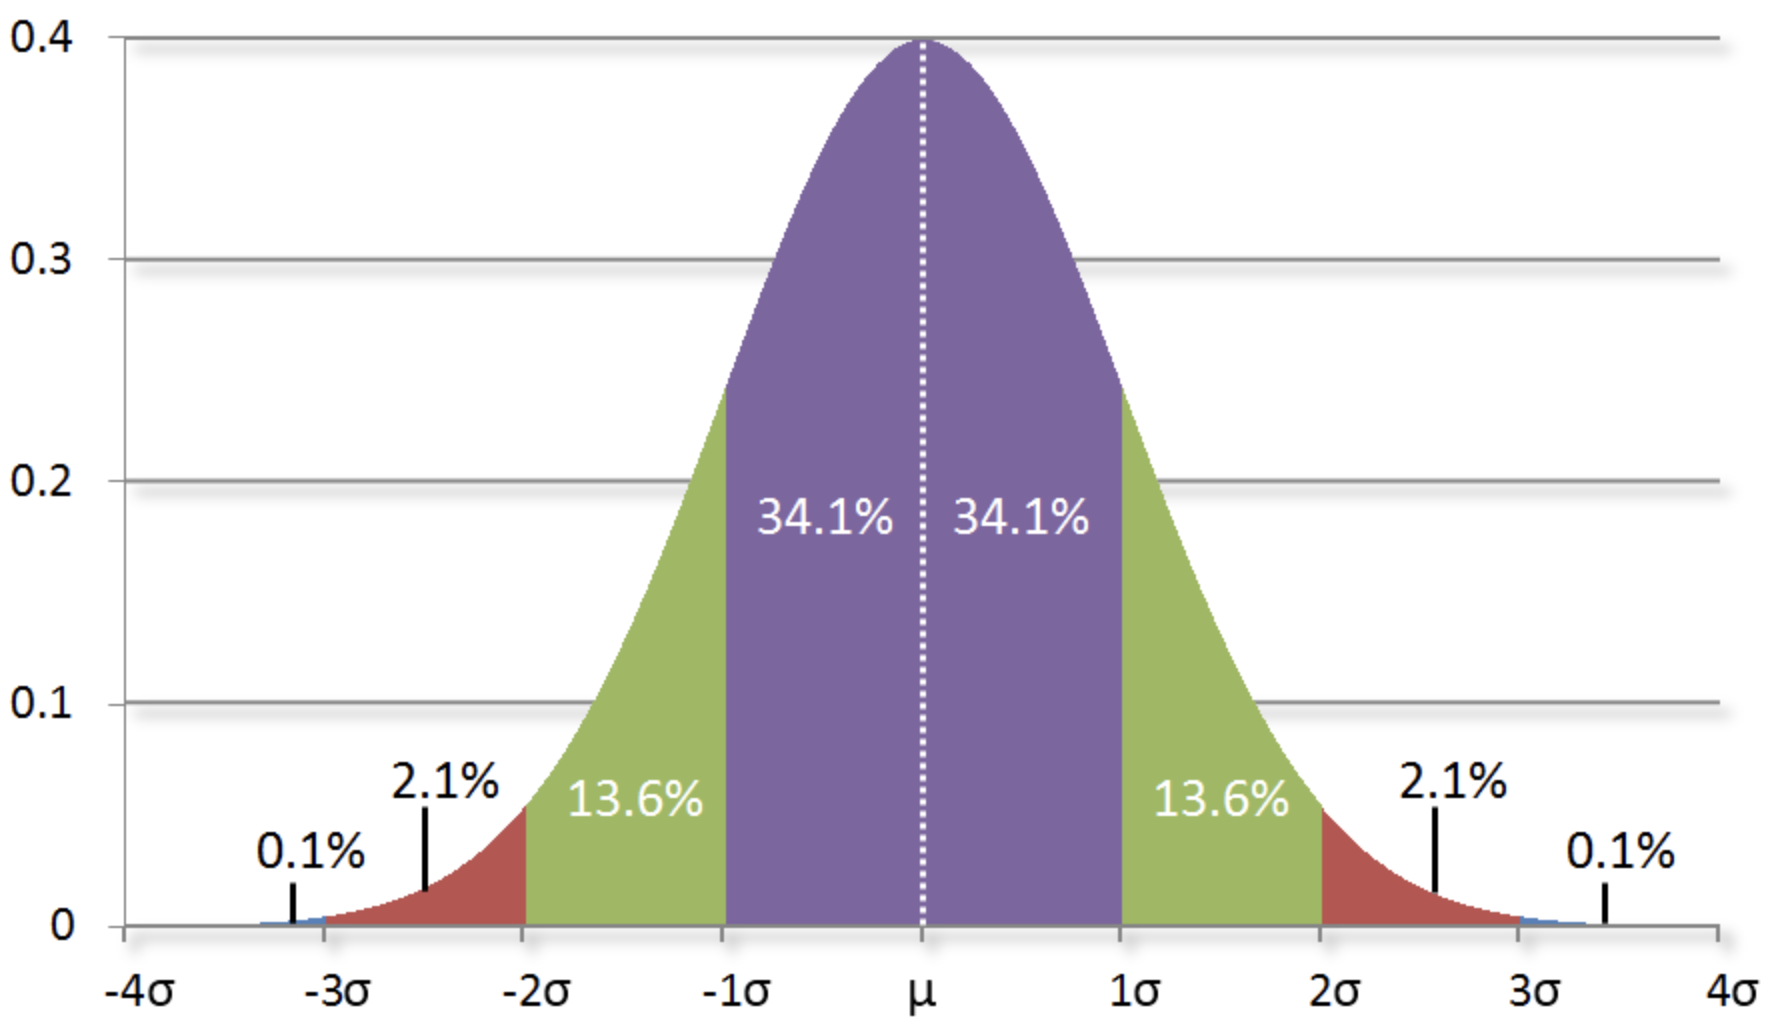
\includegraphics{Courbe_normale.png}
\caption{}
\end{figure}

Quelque soit la forme de la loi normale:

\begin{enumerate}
\def\labelenumi{\arabic{enumi}.}
\item
  L'intervalle d'un écart-type de part et d'autre de la moyenne contient
  68\% de la distribution
\item
  L'intervalle de deux écart-types de part et d'autre de la moyenne
  contient 95\% de la distribution
\item
  L'intervalle de trois écart-types de part et d'autre de la moyenne
  contient 99,7\% de la distribution
\end{enumerate}

\end{frame}

\begin{frame}{Ecart-type correspondant à x pourcentage de la
distribution}

\begin{itemize}
\tightlist
\item
  Il est préférable de partir de l'intervalle de déterminer plus
  précisément le nombre d'écart-type qui délimite l'intervalle.
\end{itemize}

\begin{itemize}[<+->]
\tightlist
\item
  Par exemple, quel intervalle contient 60\% de la distribution?
\end{itemize}

\begin{itemize}[<+->]
\tightlist
\item
  Autrement dit, comme la courbe est symétrique, on dira que 30\% de la
  distribution se trouve entre la moyenne et la valeur recherchée. Donc
  que 20\% se trouve au-delà.
\end{itemize}

\begin{itemize}[<+->]
\tightlist
\item
  Prob(distribution \textless{} v1) = 0.2 nous donne tout simplement la
  valeur de 20 ième percentile de la distribution
\end{itemize}

\begin{itemize}[<+->]
\tightlist
\item
  Prob(distribution \textless{} v2) = 0.8 dit que 80\% de la
  distribution est inférieure à cette valeur.
\end{itemize}

\begin{itemize}[<+->]
\tightlist
\item
  Donc l'intervalle {[}V1, V2{]} contient 60\% (80\% - 20\%) de la
  distribution
\end{itemize}

\end{frame}

\begin{frame}[fragile]{Ecart-type correspondant à x pourcentage de la
distribution}

On peut le calculer assez facilement avec la fonction qnorm.

\begin{Shaded}
\begin{Highlighting}[]
\NormalTok{v1 <-}\StringTok{ }\KeywordTok{qnorm}\NormalTok{(}\FloatTok{0.20}\NormalTok{, }\DataTypeTok{mean =} \DecValTok{5}\NormalTok{, }\DataTypeTok{sd =} \DecValTok{3}\NormalTok{)}
\NormalTok{v1}
\end{Highlighting}
\end{Shaded}

\begin{verbatim}
## [1] 2.475136
\end{verbatim}

\begin{Shaded}
\begin{Highlighting}[]
\NormalTok{v2 <-}\StringTok{ }\KeywordTok{qnorm}\NormalTok{(}\FloatTok{0.80}\NormalTok{, }\DataTypeTok{mean =} \DecValTok{5}\NormalTok{, }\DataTypeTok{sd =} \DecValTok{3}\NormalTok{)}
\NormalTok{v2}
\end{Highlighting}
\end{Shaded}

\begin{verbatim}
## [1] 7.524864
\end{verbatim}

\begin{itemize}[<+->]
\tightlist
\item
  Ainsi, on trouve que l'intervalle en question est {[}2,47; 7,52{]}
  pour la distribution normale N(5, 3).
\end{itemize}

\begin{itemize}[<+->]
\tightlist
\item
  Cet intervalle contient 60\% de la distribution
\end{itemize}

\end{frame}

\begin{frame}[fragile]{Ecart-type correspondant à x pourcentage de la
distribution}

\begin{Shaded}
\begin{Highlighting}[]
\KeywordTok{ggplot}\NormalTok{(}\DataTypeTok{data =} \KeywordTok{data.frame}\NormalTok{(}\DataTypeTok{x =} \KeywordTok{c}\NormalTok{(}\OperatorTok{-}\DecValTok{5}\NormalTok{, }\DecValTok{15}\NormalTok{)), }\KeywordTok{aes}\NormalTok{(x)) }\OperatorTok{+}
\StringTok{  }\KeywordTok{stat_function}\NormalTok{(}\DataTypeTok{fun =}\NormalTok{ dnorm, }\DataTypeTok{args =} \KeywordTok{list}\NormalTok{(}\DataTypeTok{mean =} \DecValTok{5}\NormalTok{, }\DataTypeTok{sd =} \DecValTok{3}\NormalTok{), }\DataTypeTok{color =} \StringTok{"red"}\NormalTok{) }\OperatorTok{+}
\StringTok{  }\KeywordTok{stat_function}\NormalTok{(}\DataTypeTok{fun =}\NormalTok{ dnorm, }\DataTypeTok{args =} \KeywordTok{list}\NormalTok{(}\DataTypeTok{mean =} \DecValTok{5}\NormalTok{, }\DataTypeTok{sd =} \DecValTok{3}\NormalTok{),}
                \DataTypeTok{geom =} \StringTok{"area"}\NormalTok{, }\DataTypeTok{fill =} \StringTok{"red"}\NormalTok{, }\DataTypeTok{xlim =} \KeywordTok{c}\NormalTok{(v1, v2), }\DataTypeTok{alpha =} \FloatTok{0.2}\NormalTok{)}
\end{Highlighting}
\end{Shaded}

\includegraphics{Séance5.2_Paramètres_variation_extension_files/figure-beamer/unnamed-chunk-5-1.pdf}

\end{frame}

\begin{frame}{Loi normale (centrée réduite)}

\begin{itemize}
\tightlist
\item
  Calculer les quantiles pour différentes distributions normales peut
  être fastidieux (dans le temps).
\item
  Alors, les statisticiens ont calculé cela pour la distribution normale
  centrée réduite
\item
  Lorsque la moyenne vaut 0 et l'écart-type vaut 1, on parle de
  distribution normale centrée réduite
\item
  Vous comprenez donc que si vous standardisez les scores de votre
  distribution normale, vous trouvez une distribution normale centrée
  réduite
\end{itemize}

\end{frame}

\begin{frame}[fragile]{Loi normale (centrée réduite)}

\begin{Shaded}
\begin{Highlighting}[]
\NormalTok{courbe_normale <-}\StringTok{ }
\StringTok{  }\KeywordTok{ggplot}\NormalTok{(}\DataTypeTok{data =} \KeywordTok{data.frame}\NormalTok{(}\DataTypeTok{x =} \KeywordTok{c}\NormalTok{(}\OperatorTok{-}\DecValTok{4}\NormalTok{, }\DecValTok{4}\NormalTok{)), }\KeywordTok{aes}\NormalTok{(x)) }\OperatorTok{+}
\StringTok{  }\KeywordTok{stat_function}\NormalTok{(}\DataTypeTok{fun =}\NormalTok{ dnorm, }\DataTypeTok{args =} \KeywordTok{list}\NormalTok{(}\DataTypeTok{mean =} \DecValTok{0}\NormalTok{, }\DataTypeTok{sd =} \DecValTok{1}\NormalTok{), }\DataTypeTok{color =} \StringTok{"blue"}\NormalTok{) }

\NormalTok{courbe_normale}
\end{Highlighting}
\end{Shaded}

\includegraphics{Séance5.2_Paramètres_variation_extension_files/figure-beamer/unnamed-chunk-6-1.pdf}

\begin{Shaded}
\begin{Highlighting}[]
\NormalTok{?dnorm}
\end{Highlighting}
\end{Shaded}

\end{frame}

\end{document}
